\section{Physics Beyond the Standard Model}

The SM is one of the most well-tested theories in physics. It had numerous
successes in predicting phenomena before they were experimentally observed. Most
recently, the Higgs boson was discovered in 2012 about five decades after the
inclusion of the BEH mechanism into the SM by Weinberg in
1967~\cite{Weinberg:1967tq}. Similarly, the gluons, $W^\pm$ and $Z$ bosons were
all predicted by the SM before direct experimental evidence for their existence
could be obtained. Despite its many successes, the SM is known to be an
incomplete theory leaving a number of phenomena unexplained:
\begin{description}

\item[Matter-antimatter asymmetry] In the Big Bang cosmological model, equal
  amounts of matter and antimatter are produced in the initial phase of the
  evolution of the universe. However, the universe observed today mostly
  consists of matter particles, thus resulting in a large asymmetry between
  matter and antimatter. The SM does not contain a mechanism that can explain
  the size of the matter-antimatter asymmetry observed in the universe.

\item[Gravitation] At the moment, no quantum field theory of gravitation exists
  that could be incorporated into the SM. Therefore, the SM does not attempt to
  describe gravitational interactions between massive particles. In addition, it
  is currently not understood why the gravitational interaction between
  elementary particles is much weaker than the strong or electroweak
  interaction.

\item[Dark matter] Based on astrophysical observations it is postulated that the
  vast majority of the universe consists of a form of matter, referred to as
  dark matter, that interacts gravitationally but not electromagnetically.

  The SM does not provide a dark matter candidate particle.

\item[]

\item[Neutrinos] Mass, Majorana, Dirac, etc.

\item[Vacuum Stability] The present minimum with a vacuum expectation
  value of $v \approx \si{246}{\GeV}$ might be either a global minimum
  in which case the universe is stable or only a local minimum which
  leads to a metastable universe. In the metastable case, the state of
  the Higgs field could tunnel to a new local or global minimum with a
  smaller vacuum expectation value. Current experimental data cannot
  distinguish whether the universe is stable or
  meta-stable\todo{citation}.

\item[Elektroweak phase transition] In baryogenesis a first order
  electroweak phase transition is needed.

\end{description}
These shortcomings do not disprove the SM, however, which still predicts and
describes many natural phenomena with excellent precision. Therefore, it is
often believed that the SM represents the low-energy manifestation of an
extended theory occurring at high energy scales, for example a \emph{Grand
  Unified Theory} that unifies the electroweak and strong interaction.


\subsection{Non-Resonant Higgs Boson Pair Production}%
\label{sec:bsm_nonresonant_hh}

Contributions of new physics might appear at energy scales beyond what can be
experimentally probed using direct searches at the LHC. However, some
sensitivity to such models is provided by indirect searches using SM processes,
which can be sensitive to heavy BSM particles via virtual corrections. These
corrections can, for example, alter the total/differential cross-section of
non-resonant \HH production. Consequently, searches for non-resonant \HH
production are already of interest, since an enhancement in its cross-section
compared to the SM expectation would be a indicator of BSM physics.

An avenue to explore BSM contributions to non-resonant \HH production is to
probe the Higgs boson self-coupling constant $\lambda_{HHH}$ for possible
deviations from the SM. Such deviations can arise through virtual corrections to
the Higgs boson self-interaction involving BSM particles as illustrated in
\Cref{fig:bsm_hh_prod_feyn}. If the mass scale of the BSM particles
participating in the virtual corrections is sufficiently large, then the
dynamics of the BSM theory can be reduced to an effective interaction vertex
between three Higgs bosons with a coupling constant
\begin{align*}
  \lambda_{HHH} = \klambda \times \lambda_{HHH}^{\text{SM}} \,\text{,}
\end{align*}
where $\lambda_{HHH}^{\text{SM}}$ is the self-coupling constant predicted by the
SM and \klambda is a coupling modifier. Due to the interference with the
$pp \to HH$ box diagram depicted in \Cref{fig:dihiggs_ggf_feyn_box}, a change in
\klambda will alter both the total cross-section of non-resonant \HH production
and the kinematic distributions of the final state particles. These effects will
be discussed in \Cref{sec:higgs_self_coupling}.

\begin{figure}[htbp]
  \centering

  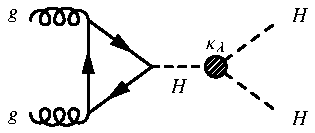
\includegraphics[width=0.35\textwidth]{feynman_graphs/di_higgs_effective}

  \caption{Non-resonant production of Higgs boson pairs for anomalous values of
    the trilinear self-coupling constant.  Contributions of new physics, for
    example through loops of heavy BSM particles, are indicated as a hatched
    circle. The effective coupling constant in units of the Higgs boson
    self-coupling constant predicted by the SM is given by \klambda.}%
  \label{fig:bsm_hh_prod_feyn}
\end{figure}

% Unitarity: Scattering probability < 1
%
% Perturbativity: Higher-order corrections become smaller as opposed to larger
On theoretical grounds, anomalous values of the Higgs boson self-coupling are
constrained to be within $|\klambda| \lessapprox 6$ derived from arguments of
unitarity and perturbativity in $HH \to HH$
scattering~\cite{DiLuzio:2017tfn}.\footnote{Similar arguments were made in the
  past to obtain upper limits on the Higgs boson mass from unitarity bounds in
  the scattering of longitudinally polarised vector bosons~\cite{Lee:1977eg}.}
These bounds still allow for a wide range of anomalous Higgs boson self-coupling
strengths, motivating experimental searches for non-resonant \HH
production. Such searches constitute a major part of
\Cref{sec:dihiggs,sec:higgs_self_coupling}, where upper limits are set on the
non-resonant \HH production cross section for a signal with SM-like kinematics
($\klambda = 1$), and for a signal with anomalous \klambda ($\klambda \neq 1$),
respectively.


\subsection{Resonant Higgs Boson Pair Production}%
\label{sec:bsm_resonant_hh}

If BSM physics appears at experimentally accessible energy scales, new particles
could be produced directly (on-shell) in collider experiments. Further assuming
that these particles are short-lived and decay into detectible SM particles, one
can reconstruct the mass of such particles from the four-momenta of their decay
products. The presence of BSM physics then appears as an enhancement of the
differential cross-section $\mathrm{d}\sigma / \mathrm{d}m$, where $m$ refers to
the invariant mass of the final state particles, in a region close to the mass
of the new particle. This phenomenon is referred to as a \emph{resonance} and
the production of particles via an intermediate resonance as \emph{resonant
  production}.

Several BSM theories extend the Higgs sector of the SM with additional scalar
particles. Provided these scalars couple to the Higgs boson and their mass
exceeds twice the Higgs boson mass, resonant production of Higgs boson pairs
would be possible. Two examples of extended Higgs sectors are outlined in the
following:
\begin{description}

\item[Additional scalar singlets] A simple extension of the SM is the addition
  of a real scalar field $\phi_{S}$ that transforms as a singlet under the SM
  gauge group. This scalar field, being a gauge singlet, does not interact with
  any of the SM fermions or vector bosons. A general choice for the potential of
  the scalar sector is~\cite{Chen:2014ask,DiMicco:2019ngk}
  \begin{align*}
    V(\phi, \phi_{S}) = V(\phi)
    + \frac{a_1}{2} (\phi^\dagger \phi) \phi_{S}
    + \frac{a_2}{2} (\phi^\dagger \phi) \phi_{S}^2
    + b_1 \phi_{S} + \frac{b_2}{2} \phi_{S}^2 + \frac{b_3}{3} \phi_{S}^3 + \frac{b_4}{4} \phi_{S}^4 \,\text{,}
  \end{align*}
  where $\phi$ refers to the complex Higgs doublet and $V(\phi)$ is the BEH
  potential. The fields can be expanded about the vacuum state according to
  $\phi = (0 \quad v + H)^{\text{T}} / \sqrt{2}$ and $\phi_{S} = v_{S} + S$,
  where $v_{S}$ is the VEV of $\phi_{S}$. After the expansion, terms bilinear in
  $H$ and $S$ appear in the potential,\footnote{The terms are non-vanishing only
    if either $a_1 \neq 0$, or $a_2 \neq 0$ and $\phi_{S}$ has non-vanishing
    VEV. See for example Ref.~\cite{Chen:2014ask}.} which indicate that the
  physical fields are mixtures of $H$ and $S$. The physical fields $H_1$ and
  $H_2$ with masses $m_1$ and $m_2$, respectively, can be expressed as
  \begin{align*}
    \begin{pmatrix}
      H_1 \\
      H_2
    \end{pmatrix}
    =
    \begin{pmatrix}
      \cos\theta & \sin\theta \\
      -\sin\theta & \cos\theta
    \end{pmatrix}
    \begin{pmatrix}
      H \\
      S
    \end{pmatrix} \,\text{,}
  \end{align*}
  with a mixing angle $\theta$. Taking $H_1$ to be the observed Higgs boson and
  $H_2$ a new scalar particle with $m_2 > 2 m_1$, processes of the form
  $pp \to H_2 \to H_1 H_1$ are possible. The production modes of $H_2$ follow
  those of the SM Higgs boson, although suppressed according to the size of the
  $H$ admixture in $H_2$.

  However, $S$ might couple to a ``hidden sector'' of
  particles which could provide suitable candidates for dark matter.


  Resonant production of SM Higgs boson pairs is predicted by several models
  with additional real scalar fields that transform as singlets under the gauge
  symmetry of the
  SM~\cite{Schabinger:2005ei,Bowen:2007ia,Barger:2007im,Dolan:2012ac,No:2013wsa,Chen:2014ask,Robens:2016xkb}

  Higgs portal models~\cite{Patt:2006fw} connects to a possible dark sector with
  particle masses similar to the SM particles via a Higgs portal.




\item[Two-Higgs-doublet-models (2HDM)]

\end{description}

~\cite{DiMicco:2019ngk}

In this thesis, the new scalar particle $X$ is assumed to have a decay width
much narrower than the experimental resolution

preferential coupling to heavy fermions such that \ggF is the dominant
production mode.

\Cref{fig:resonant_production_feyn}

\begin{figure}[htbp]
  \centering

  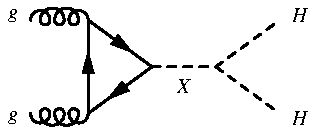
\includegraphics[width=0.35\textwidth]{feynman_graphs/di_higgs_resonant}

  \caption{Resonant production of a pair of SM Higgs bosons via an intermediate
    scalar resonance $X$ produced in \ggF.}%
  \label{fig:resonant_production_feyn}
\end{figure}







Additional singlet

Additional doublet




narrow \ggF is the dominant production mode








Provided the mass of these
particles exceeds twice the Higgs boson mass









To be reasonably model-independent, focus on scalar particles, $X$, with a decay
width much narrower than the experimental resolution produced via \ggF.

For example, such particles are predicted by models with extended Higgs
sectors. These extensions can introduce, for example, additional Higgs singlets
(Higgs portal models) or doublets (two-Higgs-doublet-models such as MSSM)


such as with additional Higgs singlets or doublets.

Extended Higgs sector

Additional singlet ()








\todo[inline]{What models predict Spin-0 resonances decaying into pair of SM
  Higgs? 2HDM}

\todo[inline]{Mention Spin-2 resonances? KK-graviton -- theoretically not favoured}

% \item[BSM] Radions, 2HDM, Warped extra dimensions, composite Higgs, hMSSM, KK
%   Gravitons: Most could decay to pairs of SM Higgs bosons.

\todo[inline]{1 page}


%%% Local Variables:
%%% mode: latex
%%% TeX-master: "../../phd_thesis"
%%% End:
